\documentclass[../main.tex]{subfiles}
\usepackage{hyperref}
\begin{document}

\section{Model Architecture}
After a thorough investigation of the TESS Dataset, we propose a \hyperref[fig:architecture]{Convolutional
Recurrent Neural Network (CRNN) architecture}.

\subsection{Input Processing}
In order to ensure uniformity across the TESS dataset, we apply a standardized
preprocessing pipeline to the raw audio signals. First, each sound bite is
resampled to a fixed rate and then normalized to a consistent amplitude. Second,
silence segments are removed to minimize irrelevant input (noise) \citep{Orhan2021}, and segmented
to a fixed length; shorter samples are padded while longer samples are trimmed.
Finally, each processed sample is converted into a Mel-spectrogram. In effect,
this transformation reduces the dimensionality of the audio data while
preserving essential information about the temporal and spectral characteristics
of the speech \citep{Orhan2021}.

\subsection{Convolutional Layers}
The CRNN architecture is initiated by a series of three-dimensional convolutional
layers designed to extract progressively abstract features from the spectrogram
input. The first block employs local feature detection, using small kernels to
capture micro-level emotional indicators and basic acoustic patterns. As the
layers deepen, the receptive fields get larger to capture broader, higher-level
abstractions, such as intonation patterns or general timbral characteristics of
certain emotions. Each convolution is followed by a max-pooling layer which
reduces the spatial dimensions of the feature maps. Moreover, batch
normalization and dropout is applied after each convolutional layer to stabilize
learning and prevent overfitting. These convolutional layers help the model ``learn effective salient features for SER and show excellent performances on several benchmark datasets'' \citep{Chen2018}.

\subsection{Recurrent Layers}
Following the convolutional layers, the model incorporates two bidirectional
Long Short-Term Memory (BiLSTM) layers. Given that the audio data in TESS is
relatively short and sequential, BiLSTMs are a practical choice as they capture
dependencies across time steps, and allow for a more nuanced understanding of
emotional expression. Additionally, the bidirectional design of the model helps
capture the full emotional arc of an utterance by analyzing past and future time
frames \citep{Orhan2021}. Thus, the RNN module serves as a temporal feature extractor \citep{Chen2018}, supporting
the objective of emotion identification over the course of the audio sample.

\subsection{Attention Mechanism}
To help the model focus on the most salient temporal features for emotion
recognition, an attention mechanism is incorporated after the BiLSTM layers \citep{Peng2020}, \citep{Chen2018}.
More precisely, the attention module calculates a weighted sum of the hidden
states from the BiLSTM, where the weights are determined by both the current hidden
state and the overall sequence of hidden states \citep{Chen2018}. This can be exceptionally
useful since it allows the model to dynamically weigh the importance of
different time steps, emphasizing parts of the audio where emotional cues are
the strongest, thus possibly improving model performance.

\subsection{Dense Layers and Output Layer}
Finally, after both the CNN and RNN modules, the resulting features are passed
through a fully-connected dense layer. This integration layer is crucial since
it combines our high-level temporal and spatial features into a single, unified
representation \citep{Chen2018}. To enhance generalization, dropout are applied within the layer.
In turn, this refined representation helps transition our data into the final
softmax output layer, producing a probability distribution across the seven
emotion classes.

\subsection{Training Protocol}
The training strategy is specifically designed around the nuanced nature of
emotional speech patterns. The model employs categorical cross-entropy loss
(standard for multi-class classification), with the Adam optimizer for its
ability to handle the inherent noise and variability in emotional expression \citep{Bhatlawande2024}.
Additionally, to enhance the robustness of the model, we apply audio-specific
data augmentation. Augmentations such as random pitch shifting and
time-stretching effectively expand our dataset by introducing slight variability
in existing data, in turn making our model less prone to overfitting \citep{Bhatlawande2024}. These protocols ensure model robustness, aiding us in our goal of building a truly useful and reliable voice-based emotion classifier.

\begin{figure}[h]
    \centering
    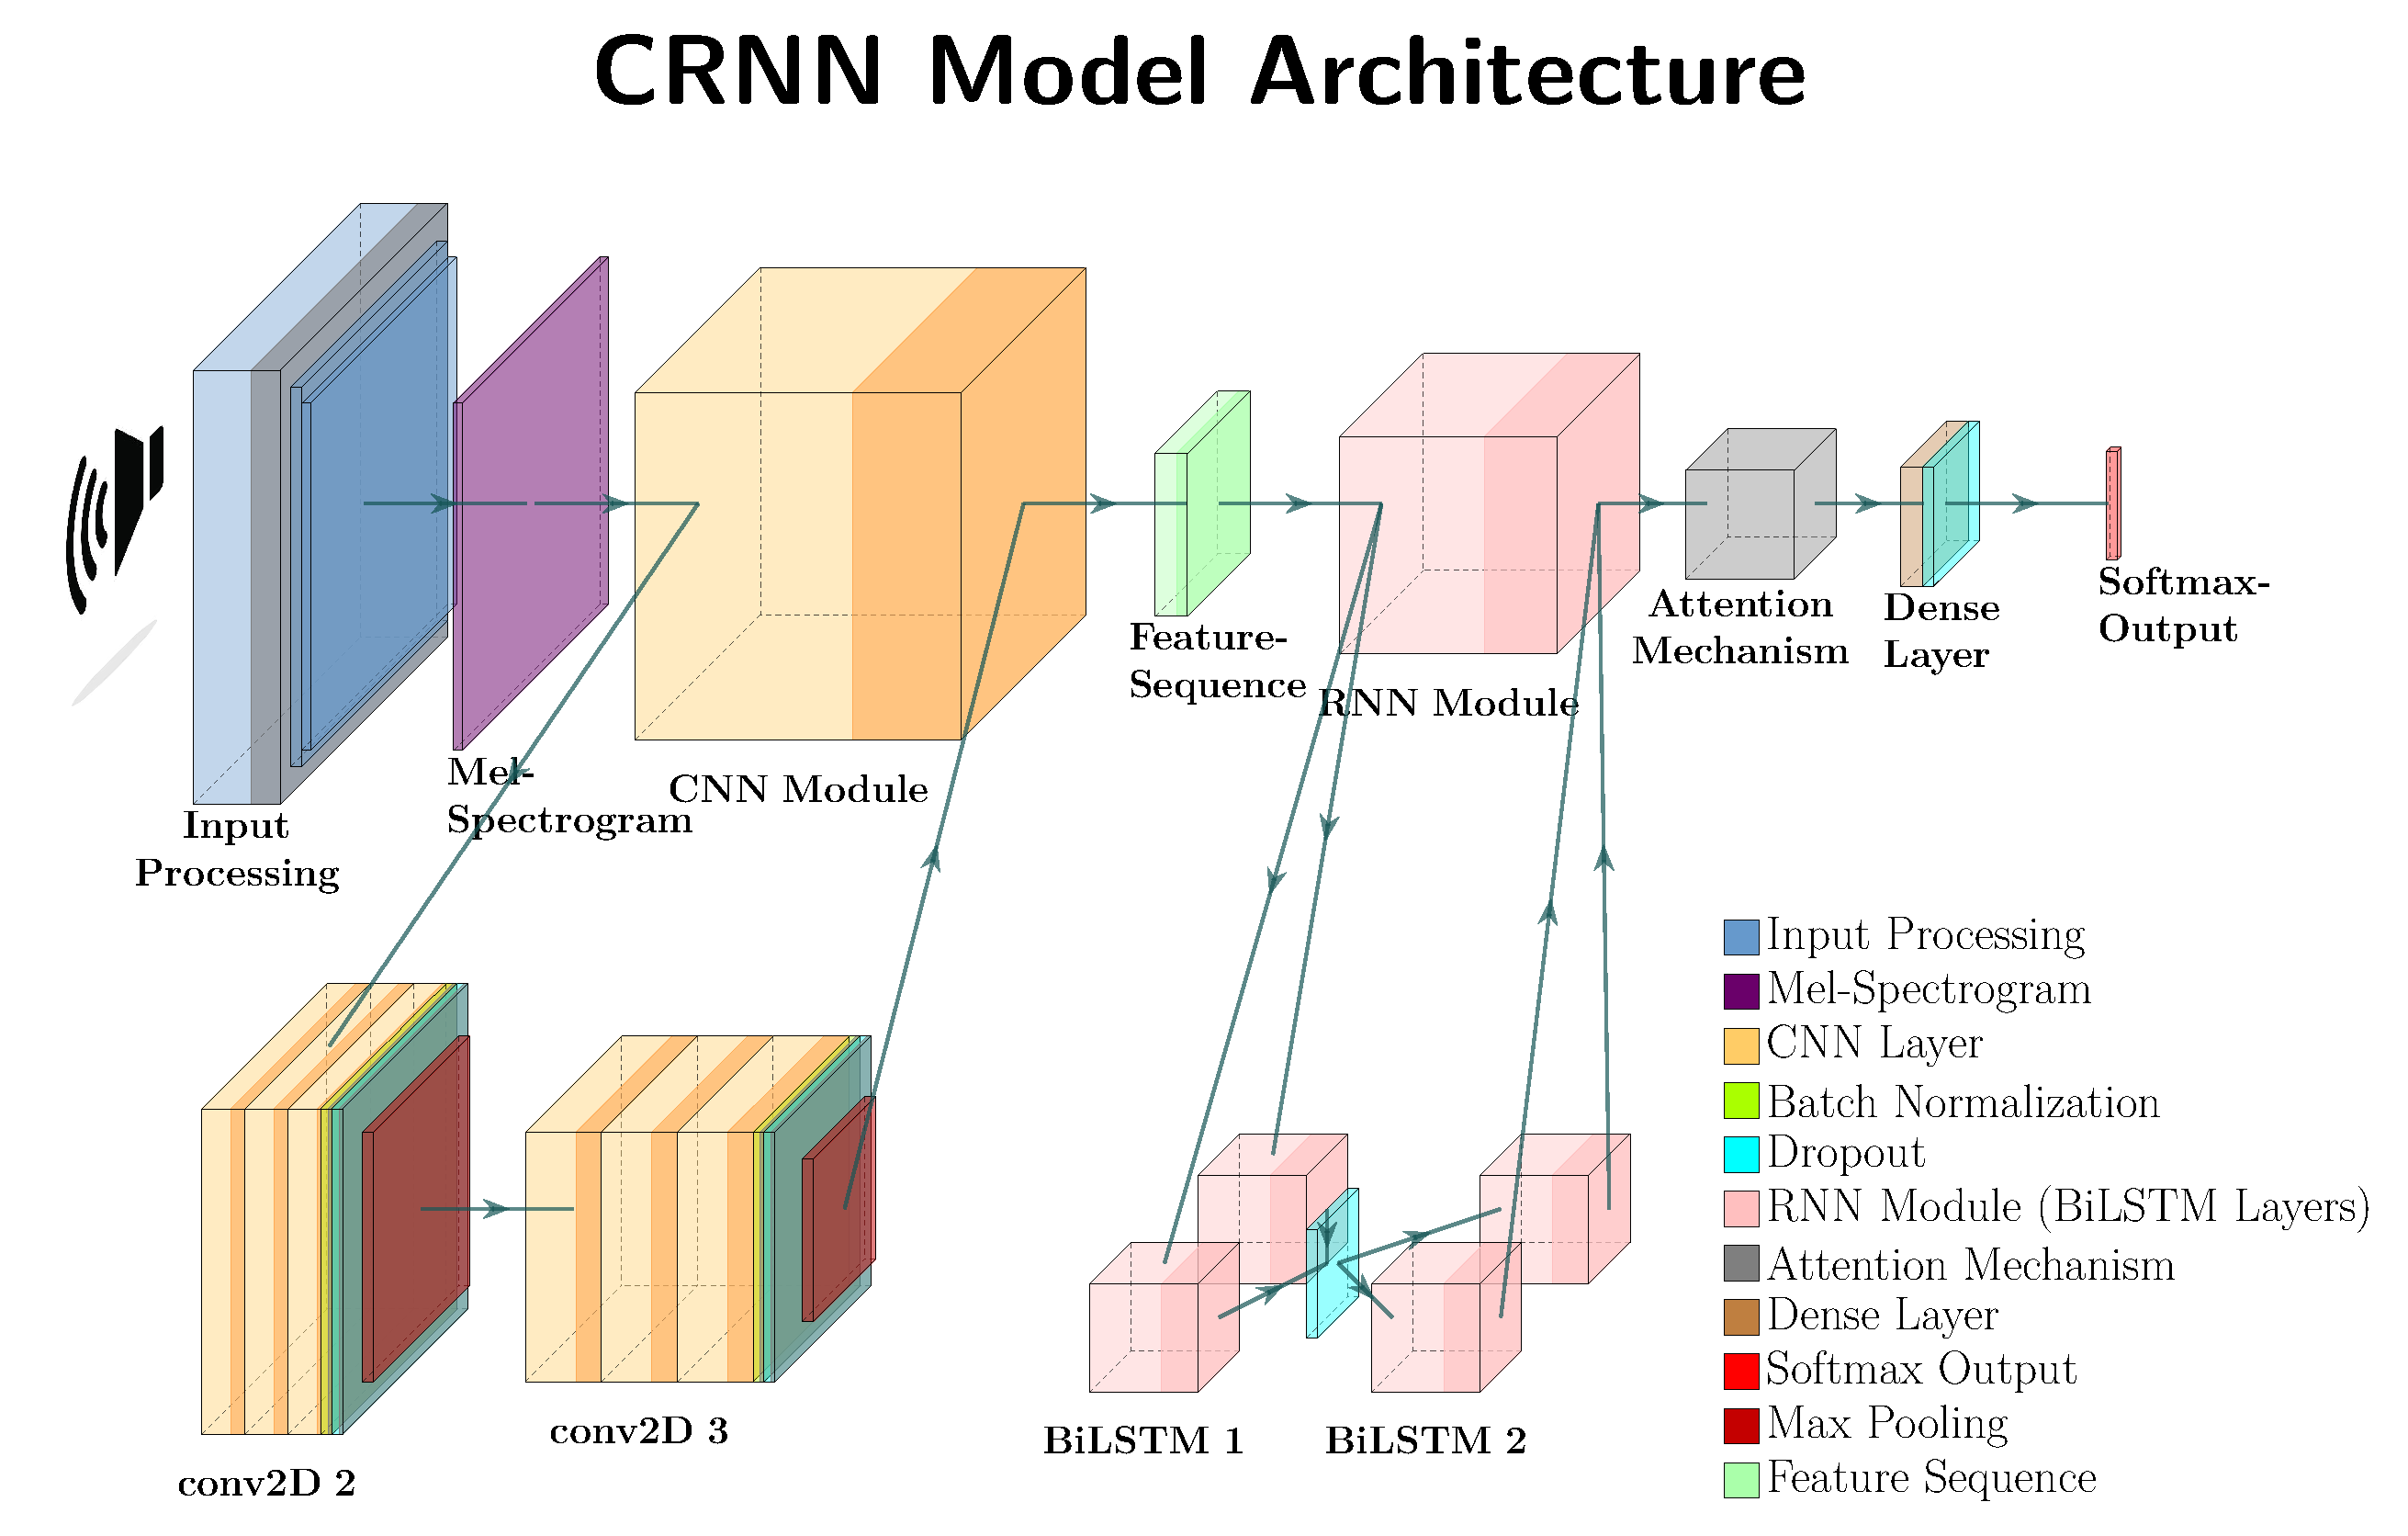
\includegraphics[width=\textwidth]{../figure/architecture_figure.pdf}
    \caption{Figure 2: Proposed CRNN Model Architecture for Emotion Classification}
    \label{fig:architecture}
\end{figure}

\end{document}
